\subsection{Proof of Correctness}  
\label{sec:proof-th1}

We now provide the proof to support the correctness of the response time analysis presented in
Theorem~\ref{theorem:general-framework}, whatever the value of vector $\vec{x}$.  %The proof strategy is to
%show that the worst-case response time of task $\tau_k$ can be safely
%upper-bounded by any assignment of $\vec{x}$ of the $k-1$
%higher-priority tasks when adopting
%Eq.~(\ref{eq:TDA-suspension-tighter0}) as the response time analysis.

Throughout the proof, we consider any arbitrary assignment
$\vec{x}$, in which $x_i$ is either $0$ or $1$. For the sake of clarity, we classify the $k-1$
higher-priority tasks into two sets: ${\bf T}_0$ and ${\bf T}_1$. A
task $\tau_i$ is in ${\bf T}_0$ if $x_i$ is $0$; otherwise, it is in
${\bf T}_1$.




Our analysis is also based on very simple properties and lemmas enunciated as follows:

\begin{Property}
\label{prop:lower-priority}
In a preemptive fixed-priority schedule, the lower-priority jobs do not impact the schedule of the higher-priority jobs.
\end{Property}

%\begin{lemma}
%\label{lemma:remove-lower-priority}
%In a preemptive fixed-priority schedule, removing a lower-priority job arrived at time $t$ does not affect the schedule of the higher-priority jobs after time $t$.
%\end{lemma}
%\begin{proof}
%This is a direct consequence of Property~\ref{prop:lower-priority}.
%\end{proof}

\begin{Lemma}
\label{lemma:remove-same-task}
In a preemptive fixed-priority schedule, if the worst-case response time of task $\tau_i$ is no more than its period $T_i$, preventing the release of a job of task $\tau_i$ does not affect the schedule of any other job of task $\tau_i$.
\end{Lemma}
\begin{proof}
Since, by assumption, the worst-case response time of task $\tau_i$ is no more than its period, any job $\tau_{i,j}$ of task $\tau_i$ completes its execution before the release of the next job $\tau_{i,j+1}$. Hence, the execution of $\tau_{i,j}$ does not directly interfere with the execution of any other job of $\tau_i$, which then depends only on the schedule of the higher priority jobs. Furthermore, as stated in Property~\ref{prop:lower-priority}, the removal of $\tau_{i,j}$ has no impact on the schedule of the higher-priority jobs, thereby implying that the other jobs of task $\tau_i$ are not affected by the removal of $\tau_{i,j}$.
\end{proof}


With the above properties, we can present the detailed proof of
Theorem~\ref{theorem:general-framework}. 

\begin{appProof}{Theorem~\ref{theorem:general-framework}}
Consider the modified task set $\tau'$ composed of $\left\{\tau_1, \tau_2, \ldots, \tau_{k-1}, \tau_k', \tau_{k+1}, \ldots \right\}$ where $\tau_k' = (C_k + S_k, 0, D_k, T_k)$. Let $\Psi$ be a schedule of $\tau'$ such that $R_k' \leq T_k$.  
Suppose that a job $J_{k}$ of task $\tau_k'$ arrives at time $r_k$ and finishes at time $f_k$. We prove that Eq.~\eqref{eq:TDA-suspension-tighter0} gives us a safe upper bound on $f_k-r_k$ for any job $J_k$ in $\Psi$.


The proof is built upon the three following steps:
\begin{enumerate}
\item We discard all the jobs that do not contribute to the response time of $J_k$ in the schedule $\Psi$. We follow an inductive strategy by iteratively inspecting the schedule of the higher priority tasks in $\Psi$, starting with $\tau_{k-1}$ until the highest priority task $\tau_1$. At each iteration, a time instant $t_j$ is identified such that $t_j \leq t_{j+1}$ ($1 \leq j < k$). Then, all the jobs of task $\tau_j$ released before $t_j$ are removed from the schedule and, if needed, replaced by an artificial job mimicking the interference caused by the residual workload of task $\tau_j$ at time $t_j$. %on the response time of job $J_k$. 
\item The final reduced schedule is analyzed so as to characterize the
  worst-case response time of $\tau_k'$ in $\Psi$. %by using workload functions.
\item We then prove that the response time analysis in Eq.~(\ref{eq:TDA-suspension-tighter0}) is indeed an upper bound on the worst-case response time $R_k'$ of $\tau_k'$.
\end{enumerate}

%!!!!!*************!!!!!!!!\\
%Since the proof involves several transformation steps. To illustrate some important steps in
%the proof, we also provide one concrete example. Consider a task
%system with 
%\begin{itemize}
%\item $T_1 = 6, C_1 = 1, S_1 = 1, x_1=1$,
%\item $T_2 = 10, C_2 = 1, S_2 = 6, x_2=0$,
%\item $T_3 = 18, C_3 = 4, S_3 = 1, x_3=1$,
%\item $T_4 = 20, C_4 = 5, S_4 = 0$.
%\end{itemize}
  
%!!!!!*************!!!!!!!!


\begin{figure*}[t]
  \centering
  
		\def\ux{0.25cm}\def\uy{0.5cm} 
		\begin{tikzpicture}[y=\uy, font=\sffamily,thick]  
		\tikzset{
			task/.style={fill=#1,  rectangle, text height=.3cm},
			task1a/.style={task=green!30},
			task1b/.style={task=green},
			task2a/.style={task=orange!30},
			task2b/.style={task=orange, minimum width=1mm},
			task3a/.style={task=pink, minimum width=1mm},
			task3b/.style={task=pink!80, minimum width=1mm},
			task4a/.style={task=cyan, minimum width=1mm},
			task4b/.style={task=cyan!50},
			task5/.style={task=blue},
			task6/.style={task=purple},
			task7/.style={minimum height=\ux,draw},
			task8/.style={minimum height=\ux,draw,thick},
			task9/.style={task=gray,minimum height=0.7cm,draw},
		}
		\tikzstyle{jobs}=[ fill=black!50];

		\begin{scope}[shift={(0,0)}]
		
		\draw[<-](2,1.1) -- (2,0);
		\draw[<->](5,1.1) -- (5,0);
		\draw[<->](8,1.1) -- (8,0);
		\draw[<->](11,1.1) -- (11,0);
		
		
		\draw[->] (0,0) node[anchor=east] {$\tau_1$}-- coordinate (xaxis) (12.5,0);

		
		\node[task7, minimum width=2*\ux,
		anchor=south west]at (2.5, 0){};
		\node[task7, minimum width=2*\ux,
		anchor=south west]at (5, 0){};
		\node[task7, minimum width=2*\ux,
		anchor=south west]at (8, 0){};
		\node[task7, minimum width=2*\ux,
		anchor=south west]at (11, 0){};
		\draw[(-), thin] (2, 0.3) -- (2.5, 0.3);

		\end{scope}
		
		
		\begin{scope}[shift={(0,-1.5)}]
		%%timeline
		
		
		\draw[<-](0,1.1) -- (0,0);
		\draw[<-](5,1.1) -- (5,0);
		\draw[<-](10,1.1) -- (10,0);
		
		
		\draw (3,0) -- (3, 0.3cm) -- (3.04, 0.3cm) --
                (3.04, 0);
		anchor=south west]  at ( 3, 0){};
		\node[task7, minimum width=2*\ux,
		anchor=south west] at (3.5, 0){};
		\node[task7, minimum width=2*\ux,
		anchor=south west] at (5.5, 0){};
		\node[task7, minimum width=2*\ux,
		anchor=south west] at (10.5, 0){};

		\draw[->] (0,0)node[anchor=east] {$\tau_2$} -- coordinate (xaxis) (12.5,0);
		\draw[(-), thin] (0, 0.3) -- (2.5, 0.3);
		\draw[(-), thin] (3.04, 0.3) -- (3.5, 0.3);
		\draw[(-), thin] (10, 0.3) -- (10.5, 0.3);
		
		
		\end{scope}

		\begin{scope}[shift={(0,-3)}]
		%%timeline
		
		\draw[<-](3,1.1) -- (3,0);
		\draw[<-](12,1.1) -- (12,0);
		

		\draw[->] (0,0)node[anchor=east] {$\tau_3$} -- coordinate (xaxis) (12.5,0);
		
		\node[task7, minimum width=4*\ux,
		anchor=south west]  at ( 4, 0){};
		\node[task7, minimum width=4*\ux,
		anchor=south west]  at ( 6, 0){};
		
		\draw[(-), thin] (3, 0.3) -- (3.5, 0.3);
		
		\end{scope}

		\begin{scope}[shift={(0,-4.5)}]
		
		
		
		\draw[->] (0,0) node[anchor=east] {$\tau_4$}-- coordinate (xaxis) (12.5,0);
		\draw[<-](3.5,1.1) -- (3.5,0)node[anchor=north] {$$};
				\node[task7, minimum width=4*\ux,anchor=south west]at (7, 0){};
		\node[task7, minimum width=6*\ux,anchor=south west]at (8.5, 0){};
		
		\foreach \x in {0,...,24}{
			\draw[-](.5*\x,0.1) -- (.5*\x,-0.1)
			node[below] {\small $\x$};
			
		}

                \draw (10, -1.5) node {\small $\rho$};
                \draw (3.5, -1.5) node {\small $t_4$};
                \draw (3, -1.5) node {\small $t_3$};
                \draw (3, -2) node {\small $t_2$};
                \draw (2, -1.5) node {\small $t_1$};
		\end{scope}
		
		\end{tikzpicture}  

\caption{An illustrative example of Step 1 in the proof of Theorem~\ref{theorem:general-framework}.}
\label{fig:example}  
\end{figure*}


\noindent{\bf Step 1: Reducing the schedule $\Psi$} 

During this step, we iteratively build an artificial schedule $\Psi^j$ from $\Psi^{j+1}$ (with $1 \leq j < k$) so that the response time of $\tau_{k}'$ remains identical. At each iteration, we define $t_j$ for task $\tau_j$ in the schedule $\Psi^{j+1}$ (with $j=k-1, k-2, \ldots, 1$) and build $\Psi^j$ by removing all the jobs released by $\tau_j$ before $t_j$.


\noindent\textit{Basic step (definition of $\Psi^k$ and $t_k$):} 

Recall that the job $J_{k}$ of task $\tau_k'$ arrives at time $r_k$ and finishes at time $f_k$ in schedule $\Psi$. We know by Property~\ref{prop:lower-priority} that the lower priority tasks $\tau_{k+1}, \tau_{k+2}, \ldots, \tau_n$ do not impact the response time of $J_{k}$. Moreover, since we assume that the worst-case response time of task $\tau_k'$ is no more than $T_k$, Lemma~\ref{lemma:remove-same-task} proves that removing all the jobs of task $\tau_k'$ but $J_{k}$ has no impact on the schedule of $J_{k}$. Therefore, let $\Psi^k$ be a schedule identical to $\Psi$ but removing all the jobs released by the lower priority tasks $\tau_{k+1}, \ldots, \tau_n$ as well as all the jobs released by $\tau_k'$ at the exception of $J_{k}$. The response time of $J_{k}$ in $\Psi^{k}$ is identical to the response time of $J_{k}$ in $\Psi$.

We define $t_k$ as the release time of $J_k$ (i.e., $t_k = r_k$).


\noindent\textit{Induction step (definition of $\Psi^j$ and $t_j$ with $1 \leq j < k$):}

Let $r_j$ be the arrival time of the last job released by $\tau_j$ before $t_{j+1}$ in $\Psi^{j+1}$ and let $J_{j}$ denote that job. %There are a two possible cases:
%\begin{itemize}
%\item $J_{j}$ completed its execution no later than $t_{j+1}$. Then, we simply set $t_j$ to $t_{j+1}$ and generate $\Psi^j$ by removing all the jobs of task $\tau_j$ arrived before $t_{j+1}$ in the schedule $\Psi^{j+1}$. By Lemma~\ref{lemma:remove-same-task} and Property \ref{prop:lower-priority}, removing all the jobs of task $\tau_j$ arrived before $t_{j+1}$ has no impact on the schedule of the higher-priority jobs (jobs released by $\tau_1, \ldots, \tau_{j-1}$) and the jobs of $\tau_j$ released after $t_{j+1}$. Moreover, because no task with a priority lower than $\tau_j$ executes jobs before $t_{j+1}$ in $\Psi^{j+1}$, removing the jobs released by $\tau_j$ before $t_{j+1}$ does not impact the schedule of the jobs of $\tau_{j+1}, \ldots, \tau_{k}$. The response time of $J_{k}$ in $\Psi^j$ thus remains unchanged in comparison to its response time in $\Psi^{j+1}$. 
%\item $J_{j}$ did not complete its execution before $t_{j+1}$.
Removing all the jobs of task $\tau_j$ arrived before $r_j$ has no impact on the schedule of any other job released by $\tau_j$ (Lemma~\ref{lemma:remove-same-task}) or any higher priority job released by $\tau_1, \ldots, \tau_{j-1}$ (Property \ref{prop:lower-priority}). Moreover, because by construction of $\Psi^{j+1}$, no task with a priority lower than $\tau_j$ executes jobs before $t_{j+1}$ in $\Psi^{j+1}$, removing the jobs released by $\tau_j$ before $t_{j+1}$ does not impact the schedule of the jobs of $\tau_{j+1}, \ldots, \tau_{k}$. Therefore, we can safely remove all the jobs of task $\tau_j$ arrived before $r_j$ without impacting the response time of $J_{k}$. Two cases must then be considered:
\begin{enumerate}[(a)]
\item $\tau_j \in {\bf T}_1$. In this case, we analyze two different subcases:
\begin{itemize}
\item $J_{j}$ did not complete its execution by $t_{j+1}$. For such a case, $t_{j}$ is set to $r_j$ and hence $\Psi^j$ is built from $\Psi^{j+1}$ by removing all the jobs released by $\tau_j$ before $r_j$.
\item $J_{j}$ completed its execution before or at $t_{j+1}$. By Lemma~\ref{lemma:remove-same-task} and Property \ref{prop:lower-priority}, removing all the jobs of task $\tau_j$ arrived before $t_{j+1}$ has no impact on the schedule of the higher-priority jobs (jobs released by $\tau_1, \ldots, \tau_{j-1}$) and the jobs of $\tau_j$ released after or at $t_{j+1}$. 
Moreover, because no task with lower priority than $\tau_j$ executes jobs before $t_{j+1}$ in $\Psi^{j+1}$, removing the jobs released by $\tau_j$ before $t_{j+1}$ does not impact the schedule of the jobs of $\tau_{j+1}, \ldots, \tau_{k}$. Therefore, $t_j$ is set to $t_{j+1}$ and $\Psi^j$ is generated by removing all the jobs of task $\tau_j$ arrived before $t_{j+1}$. The response time of $J_{k}$ in $\Psi^j$ thus remains unchanged in comparison to its response time in $\Psi^{j+1}$.  
\end{itemize}
\item $\tau_j \in {\bf T}_0$. For such a case, we set $t_{j}$ to $t_{j+1}$. Let $c_j^*$ be the remaining execution time for the job of task $\tau_j$ at time $t_j$. We know that $c_j^*$ is at most $C_j$. Since by construction of $\Psi^j$, all the jobs of $\tau_j$ released before $t_j$ are removed, the job of task $\tau_j$ arrived at time $r_j$ ($< t_j$) is replaced by a new job released at time $t_j$ with execution time $c_j^*$ and the same priority than $\tau_j$. Clearly, this has no impact on the execution of any job executed after $t_j$ and thus on the response time of $J_k$. The remaining execution time $c_j^*$ of $\tau_j$ at time $t_j$ is called the \emph{residual workload} of task $\tau_j$ in the rest of the proof.
\end{enumerate}
%\end{itemize}
 
This iterative process is repeated until producing $\Psi^1$. The procedures are well-defined and it is therefore guaranteed that $\Psi^1$ can be constructed. Note that after each iteration, the number of jobs considered in the resulting schedule has been reduced, yet without affecting the response time of $J_k$.

 


\begin{example}
Consider the 4 tasks $\tau_1 =(1,1,6,6)$, $\tau_2 =(1,6,10,10)$, $\tau_3 =(4,1,18,18)$ and $\tau_4 =(5,0,20,20)$.

Figure~\ref{fig:example} depicts a possible schedule of those tasks. We assume that the first job of task $\tau_1$ arrives
at time $4+\epsilon$ with a very small $\epsilon > 0$. The first job
of task $\tau_2$ suspends itself from time $0$ to time $5+\epsilon$,
and is blocked by task $\tau_1$ from time $5+\epsilon$ to time
$6+\epsilon$. After some very short computation with $\epsilon$ amount
of time, the first job of task $\tau_2$ suspends itself again from
time $6+2\epsilon$ to $7$. 
   
In the schedule illustrated in Figure~\ref{fig:example}, $f_4$ is $20-\epsilon$.
We define $t_4$ as $7$. Then, we set $t_3$ to $6$. When considering
task $\tau_2$, since it belongs to ${\bf T}_0$, we greedily set $t_2$
to $t_3=6$ and the residual workload $c_2^*$ is $1$. Then, $t_1$ is set
to $4+\epsilon$. In the above schedule, the idle time from
$4+\epsilon$ to $20-\epsilon$ is at most $2 = S_1+S_3$. We have to
further consider one job of task $\tau_2$ arrived before time $t_1$
with execution time $C_2$.
\end{example}


\begin{Lemma}
\label{lem:max_idle}
Let $\sigma_j$ be the amount of time during which the processor remains idle within $[t_j, t_{j+1})$ in $\Psi^1$. It holds that $\sum_{j=1}^{i-1} \sigma_j \leq \sum_{j=1}^{i-1} x_j S_j$. %$\sigma_j \leq S_j$.
\end{Lemma}
\begin{proof}
If $t_j = t_{j+1}$, which is the case when $x_j = 0$ (see Case (b) of the reduction process), then $\sigma_j$ is obviously equal to $0$. 

If $t_j \not= t_{j+1}$, then we are in subcase 1 of Case (a) of the schedule reduction process (i.e., when $x_j = 1$). In that case, $t_j = r_j$ and the job $J_j$ did not complete its execution yet. Therefore, the amount of time during which the processor may remain idle within $[t_j, t_{j+1})$ is at most $S_j$ time units. 

From those two cases, it results that $\sum_{j=1}^{i-1} \sigma_j = \sum_{j=1}^{i-1} x_j \sigma_j \leq \sum_{j=1}^{i-1} x_j S_j$.
\end{proof}

\noindent{\bf Step 2: Analyzing the final reduced schedule $\Psi^1$}


We now analyze the properties of the final schedule $\Psi^1$ in which all the unnecessary jobs have been removed. 


The proof is based on the fact that for any interval $[t_1, t)$, there is 
\begin{equation}
\label{eq:exec_plus_idle}
\operatorname{idle}(t_1, t) + \operatorname{exec}(t_1, t)  = (t - t_1)
\end{equation}
where $\operatorname{exec}(t_1, t)$ is the amount of time during which the processor executes tasks within $[t_1, t)$, and $\operatorname{idle}(t_1, t)$ is the amount of time during which the processor remains idle within the interval $[t_1, t)$.

%If $t_i < t_{i+1}$, the processor may idle in the time interval $[t_i,
%t_{i+1})$ in $\Psi^1$. 
%Let $\sigma_i$ be the total idle time in $\Psi^1$ within the time interval $[t_i, t_{i+1})$. 

From Lemma~\ref{lem:max_idle}, it holds that
\begin{align}
\label{eq:sumof-sigma}
%\operatorname{idle}(t_1, t) \leq \sum_{i: t_i < t} \sigma_i
\operatorname{idle}(t_1, t) \leq \sum_{j=1}^{i-1} x_j S_j.
\end{align}
%From Lemma~\ref{lem:max_idle}. %If $t_i$ is equal to $t_{i+1}$, then $\sigma_i$ is set to $0$. 


Because there is no job released by lower priority tasks than
$\tau_k'$ in $\Psi^1$, we only focus on the execution patterns of the
tasks $(\tau_1, \tau_2, \ldots, \tau_{k-1}, \tau_k')$. According to
Step 1, we should consider two cases:
\begin{itemize}
\item $\tau_j \in {\bf T}_1$. This corresponds to Case
  (a) in Step 1, which tells us that there is no job of task $\tau_j$ arrived
  before $t_j$ in $\Psi^1$.   In this case, for any $\Delta \geq 0$, the workload $W_j^1(\Delta)$, executed by
  $\tau_j$ on the processor from $t_j$ to $t_j+\Delta$ is upper bounded by
\begin{equation}
  \label{eq:execution-case1}
  W_j^1(\Delta) = \floor{\frac{\Delta}{T_j}}C_j + \min\left\{\Delta-\floor{\frac{\Delta}{T_j}}T_j, C_j\right\}.
\end{equation}
\item $\tau_j \in {\bf T}_0$. This
  corresponds to case (b) in Step 1, which tells us that there might be a job arrived
  before $t_j$ with a residual workload $c_j^*$ at time $t_j$. %In this case, for any $\Delta
  %\geq 0$, the workload $\widehat{W}_j^0(\Delta, c_j^*)$ executed by $\tau_j$ from $t_j$ to $t_j+\Delta$ has to consider 
  %Two subcases are considered:
  %\begin{itemize}
  %\item If the residual workload $c_j^*$
  %of task $\tau_j$ is $0$, the earliest next arrival time of task $\tau_j$
  %can be any time instant at or after $t_j$. 
%In this case, for any $\Delta \geq 0$, the workload $\widehat{W}_j^0(\Delta, c_j^*)$ executed by $\tau_j$ from $t_j$ to $t_j+\Delta$ is upper bounded by $W_j^1(\Delta)$. 
%\item If the residual workload $c_j^*$ of task $\tau_j$ is larger than $0$,
  Let $c_j^*$ be the residual workload of task $\tau_j$ at $t_j$. 
  Since by assumption $\tau_j$ respects all its deadlines, the absolute deadline of the job of $\tau_j$ active at $t_j$ must be at least $t_j + c_j^*$; otherwise that job would miss its
  deadline. Therefore, the earliest arrival time of task $\tau_j$
  arriving \emph{strictly after $t_j$} is at least $t_j + (T_j-D_j +
  c_j^*)$. For notational brevity, let $\rho_j$ be
  $(T_j-D_j + c_j^*)$. In this case, for any $\Delta \geq 0$ and $c_j^* > 0$, the workload $\widehat{W}_j^0(\Delta, c_j^*)$ executed by $\tau_j$ from $t_j$ to $t_j+\Delta$ is upper bounded by
  \begin{equation}
  \label{eq:execution-case2-precise}
  \widehat{W}_j^0(\Delta, c_j^*)=
  \begin{cases}
    \Delta & \mbox{ if } \Delta \leq  c_j^*\\
    c_j^* & \mbox{ if } c_j^* < \Delta \leq  \rho_j\\
   c_j^* + W_j^1(\Delta-\rho_j) & \mbox{ otherwise}.
  \end{cases}
\end{equation}
%\end{itemize}
%It is proved in Lemma~\ref{lemma:Wj0-dominate} that the worst case
%residual workload in $\widehat{W}_j^0(\Delta, c_j^*)$ by considering
%both Eq.~(\ref{eq:execution-case2-precise0}) and
%Eq.~(\ref{eq:execution-case2-precise}) 
%is to have $c_j^* = C_j$, i.e.,

It is easy to see that Eq.~\eqref{eq:execution-case2-precise} is maximized when $c_j^*$ is maximum, that is, when $c_j^* = C_j$. It results that for all $\Delta \geq 0$, we have $\widehat{W}_j^0(\Delta, C_j) \geq
\widehat{W}_j^0(\Delta, c_j^*)$. For the sake of notational brevity, for the rest of this prove, we use the notation $W_j^0(\Delta)$ to denote $\widehat{W}_j^0(\Delta, C_j)$.

%For the sake of notational brevity,
%we introduce the notation $W_j^0(\Delta)$ defined as follows.
%\begin{equation}
%  \label{eq:execution-case2-upperbounded}
% W_j^0(\Delta) \equals \widehat{W}_j^0(\Delta, C_j) 
%\end{equation}
\end{itemize}

Summing the workloads of the tasks in ${\bf T}_0$ and ${\bf T}_1$, we have
for $i=2,3,\ldots,k-1$ that $\forall t \mid t_{i-1} \leq t < t_i$
\begin{align}
\label{eq:exec_time}
\operatorname{exec}(t_1, t) \leq \sum_{j=1}^{i-1} x_j\cdot W_j^1(t-t_j)  + (1-x_j)\cdot W_j^0(t-t_j).
\end{align}

Injecting Eqs.~(\ref{eq:sumof-sigma}) and (\ref{eq:exec_time}) in Eq.~(\ref{eq:exec_plus_idle}), we have
for $i=2,3,\ldots,k-1$ that $\forall t \mid t_{i-1} \leq t < t_i$
\begin{equation}
\label{eq:exec_plus_idle-2}
\sum_{j=1}^{i-1} x_j\cdot (W_j^1(t-t_j) +\sigma_j) + (1-x_j)\cdot W_j^0(t-t_j) \geq t-t_1.
\end{equation}
Moreover, since $\tau_k'$ does not complete its execution before $f_k$ and because, by definition, $\tau_k'$ does not self-suspend, it holds that $\forall t \mid t_k \leq t < f_k$,
\begin{equation}
\label{eq:exec_plus_idle-3}
C'_k +\sum_{j=1}^{k-1} x_j\cdot (W_j^1(t-t_j) +\sigma_j) + (1-x_j)\cdot W_j^0(t-t_j) > t-t_1.
\end{equation}

\begin{example}
Consider the same 4 tasks as in Example~\ref{ex:proof_step1}, for which a possible schedule was depicted in Figure~\ref{fig:example}. We have $\sigma_1=1$, $\sigma_2=0$ and $\sigma_3=1$. The corresponding functions
$W_1^1(t-t_1)$, $W_2^0(t-t_2)$, $W_3^1(t-t_3)$ are illustrated in
Figure~\ref{fig:example-step2}. Therefore, it is rather clear that all
the conditions in Eq.~\eqref{eq:exec_plus_idle-2} and
Eq.~\eqref{eq:exec_plus_idle-3} hold by simple arithmetics.
\end{example}


\begin{figure}[t]
  \centering

		\def\ux{0.32cm}\def\uy{0.5cm} 
		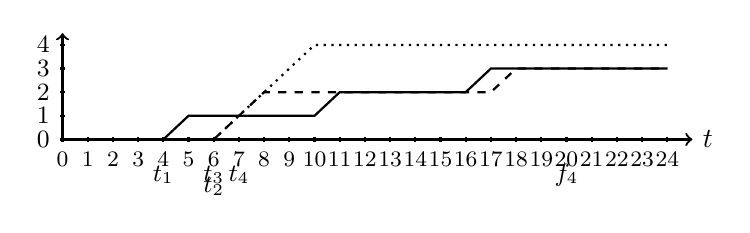
\begin{tikzpicture}[x=\ux,y=\uy, font=\sffamily,thick]  
		\tikzset{
			task/.style={fill=#1,  rectangle, text height=.3cm},
			task1a/.style={task=green!30},
			task1b/.style={task=green},
			task2a/.style={task=orange!30},
			task2b/.style={task=orange, minimum width=1mm},
			task3a/.style={task=pink, minimum width=1mm},
			task3b/.style={task=pink!80, minimum width=1mm},
			task4a/.style={task=cyan, minimum width=1mm},
			task4b/.style={task=cyan!50},
			task5/.style={task=blue},
			task6/.style={task=purple},
			task7/.style={minimum height=\ux,draw},
			task8/.style={minimum height=\ux,draw,thick},
			task9/.style={task=gray,minimum height=0.7cm,draw},
		}
		\tikzstyle{jobs}=[ fill=black!50];
		
		\draw[->] (0,0) -- coordinate (xaxis) (25,0) node[anchor=west] {$t$};
		\foreach \x in {0,...,24}{
			\draw[-](\x,0.1) -- (\x,-0.1)
			node[below] {\footnotesize $\x$};
			
		}
		\draw[->] (0,0) node[anchor=east] {}-- coordinate (xaxis) (0,4.5);
		\foreach \y in {0,...,4}{
			\draw[-](0.1, \y) -- (-0.1, \y)
			node[left] {\small $\y$};
			
		}

                \draw (20, -1.5) node {\small $f_4$};
                \draw (7, -1.5) node {\small $t_4$};
                \draw (6, -1.5) node {\small $t_3$};
                \draw (6, -2) node {\small $t_2$};
                \draw (4, -1.5) node {\small $t_1$};

                \draw[-,thick] (4,0) -- (5, 1) -- (10, 1) -- (11, 2) -- (16, 2)
                -- (17, 3) -- (22, 3) -- (23, 3) -- (24, 3);
                \draw[-,dashed] (6,0) -- (7, 1) -- (8, 2) -- (17, 2) -- (18, 3)
                -- (24, 3);
                \draw[-,dotted] (6,0) -- (10, 4) -- (24, 4);
		\end{tikzpicture}    
  \caption{The workload function for the three higher-priority tasks in Figure~\ref{fig:example-step2}. Solid line: $W_1^1(t-t_1)$, Dashed line: $W_2^0(t-t_2)$, Dotted line: $W_3^1(t-t_3)$, where the functions are $0$ if $t-t_j < 0$ for $j=1,2,3$.}
  \label{fig:example-step2}
\end{figure}

\noindent{\bf Step 3: Creating a Safe Response-Time Upper Bound}


\begin{figure*}[t]
  \centering

		\def\ux{0.25cm}\def\uy{0.5cm} 
		\begin{tikzpicture}[y=\uy, font=\sffamily,thick]  
		\tikzset{
			task/.style={fill=#1,  rectangle, text height=.3cm},
			task1a/.style={task=green!30},
			task1b/.style={task=green},
			task2a/.style={task=orange!30},
			task2b/.style={task=orange, minimum width=1mm},
			task3a/.style={task=pink, minimum width=1mm},
			task3b/.style={task=pink!80, minimum width=1mm},
			task4a/.style={task=cyan, minimum width=1mm},
			task4b/.style={task=cyan!50},
			task5/.style={task=blue},
			task6/.style={task=purple},
			task7/.style={minimum height=\ux,draw},
			task8/.style={minimum height=\ux,draw,thick},
			task9/.style={task=gray,minimum height=0.7cm,draw},
		}
		\tikzstyle{jobs}=[ fill=black!50];

		\begin{scope}[shift={(0,0)}]
		
		\draw[<-](2,1.1) -- (2,0);
		\draw[<-](5,1.1) -- (5,0);
		\draw[<-](8,1.1) -- (8,0);
		\draw[<-](11,1.1) -- (11,0);
		
		
		\draw[->] (0,0) node[anchor=east] {$\tau_1$}-- coordinate (xaxis) (12.5,0);

		
		\node[task7, minimum width=2*\ux,
		anchor=south west]at (3, 0){};
		\node[task7, minimum width=2*\ux,
		anchor=south west]at (5, 0){};
		\node[task7, minimum width=2*\ux,
		anchor=south west]at (8, 0){};
		\node[task7, minimum width=2*\ux,
		anchor=south west]at (11, 0){};
		\draw[(-), thin] (2, 1.5) -- (3, 1.5);
		\node[anchor=south] at (2.5, 1.5) {$\sum_{i=1}^{k-1} x_i \cdot \sigma_i=2$};

		\end{scope}
		
		
		\begin{scope}[shift={(0,-1.5)}]
		%%timeline
		
		
		\draw[<-](2.5,1.1) -- (2.5,0);
		\draw[<-](3,1.1) -- (3,0);
		\draw[<-](8,1.1) -- (8,0);
		
		
		\node[task7, minimum width=2*\ux,
		anchor=south west] at (3.5, 0){};
		\node[task7, minimum width=2*\ux,
		anchor=south west] at (4, 0){};
		\node[task7, minimum width=2*\ux,
		anchor=south west] at (8.5, 0){};

		\draw[->] (0,0)node[anchor=east] {$\tau_2$} -- coordinate (xaxis) (12.5,0);
		
		
		\end{scope}

		\begin{scope}[shift={(0,-3)}]
		%%timeline
		
		\draw[<-](2.5,1.1) -- (2.5,0);
		\draw[<-](11.5,1.1) -- (11.5,0);
		

		\draw[->] (0,0)node[anchor=east] {$\tau_3$} -- coordinate (xaxis) (12.5,0);
		
		\node[task7, minimum width=2*\ux,
		anchor=south west]  at ( 4.5, 0){};
		\node[task7, minimum width=6*\ux,
		anchor=south west]  at ( 5.5, 0){};
		
		\end{scope}

		\begin{scope}[shift={(0,-4.5)}]
		\draw[->] (0,0) node[anchor=east] {$\tau_4$}-- coordinate (xaxis) (12.5,0);
		\draw[<-](3.5,1.1) -- (3.5,0)node[anchor=north] {$$};
				\node[task7, minimum width=4*\ux,anchor=south west]at (7, 0){};
		\node[task7, minimum width=6*\ux,anchor=south west]at (9, 0){};
		
		\foreach \x in {0,...,24}{
			\draw[-](.5*\x,0.1) -- (.5*\x,-0.1)
			node[below] {\small $\x$};
			
		}

                \draw (10, -1.5) node {\small $f_4$};
                \draw (3, -1.5) node {\small $t_4^*$};
                \draw (3.5, -1.5) node {\small $t_4$};
                \draw (2.5, -1.5) node {\small $t_3^*$};
                \draw (2.5, -2.2) node {\small $t_2^*$};
                \draw (2, -1.5) node {\small $t_1^*$};
		\end{scope}
		
		\end{tikzpicture}  

\caption{An illustrative example of Step 3 in the proof of Theorem~\ref{theorem:general-framework} based on an \emph{imaginary} schedule.}
\label{fig:example-proof-final}  
\end{figure*}

This step constructs a safe response-time analysis based on the
conditions in Eqs.~(\ref{eq:exec_plus_idle-2}) and
(\ref{eq:exec_plus_idle-3}). We will construct another release pattern
which moves $t_i$ to $t_i^*$ for $i=2,3,\ldots,k$ such that $t_i^*
\leq t_i$ and the corresponding conditions in Eqs.~(\ref{eq:exec_plus_idle-2}) and
(\ref{eq:exec_plus_idle-3}) will become worse when we use $t_i^*$. We start
the procedure as follows:
\begin{itemize}
\item Initial Step: Let $t_1^*$ be $t_1$.
\item Iterative steps ($i=2,3,\ldots,k$): Let $t_i^*$ be $t_{i-1}^*+x_{i-1}\cdot\sigma_{i-1}$.
\end{itemize}
This results in $t_i^* \leq t_i$ for $i=2,3,\ldots,k$. Moreover, by
definition, $t_j^*$ is $t_1^* + \sum_{i=1}^{j-1} x_i\cdot\sigma_i$ for
$j=2,3,\ldots,k$.
For any task $\tau_j$ in ${\bf T}_1$,  $\forall \Delta \geq 0$, since $t_j \geq t_j^*$, we have
\begin{equation}
  \label{eq:execution-case1-shifted}
  W_j^1(\Delta)  \leq W_j^1(\Delta + (t_j-t_j^*)).
\end{equation}
For any task $\tau_j$ in ${\bf T}_0$,  $\forall \Delta \geq 0$, since $t_j \geq t_j^*$, we have
\begin{equation}
  \label{eq:execution-case2-shifted}
  W_j^0(\Delta)  \leq W_j^0(\Delta + (t_j-t_j^*)).
\end{equation}

Therefore, for any $j=1,2,\ldots,k-1$, the contribution $W_j^1(t-t_j)
\leq W_j^1(t-t_j^*)$ and $W_j^0(t-t_j) \leq W_j^0(t-t_j^*)$ for any $t
\geq t_j$. Putting these into 
Eqs.~(\ref{eq:exec_plus_idle-2}) $\forall t \mid t_k^* \leq t < t_k$ leads to
{\small \begin{align}
&\sum_{j=1}^{k-1} x_j\cdot (W_j^1(t-t_j^*)+\sigma_j) + (1-x_j)\cdot W_j^0(t-t_j^*) \geq t-t_1,\nonumber\\
\Rightarrow& \sum_{j=1}^{k-1} x_j\cdot W_j^1(t-t_j^*) + (1-x_j)\cdot W_j^0(t-t_j^*) \geq t-t_k^*.
\label{eq:exec_plus_idle-4}
\end{align}}
Similarly, putting these into 
Eqs.~(\ref{eq:exec_plus_idle-3}) $\forall t \mid t_k \leq t < f_k$ leads to 
\begin{equation}
\label{eq:exec_plus_idle-5}
C_k'+\sum_{j=1}^{k-1} x_j\cdot W_j^1(t-t_j^*) + (1-x_j)\cdot W_j^0(t-t_j^*) > t-t_k^*.
\end{equation}
 By the assumption that $C_k' \geq C_k > 0$, we can unify the above inequalities in Eq.~(\ref{eq:exec_plus_idle-4}) and Eq.~(\ref{eq:exec_plus_idle-5}) as follows:
$\forall t \mid t_k^* \leq t < f_k$
\begin{equation}
\label{eq:exec_plus_idle-almost-final} 
C_k'+\sum_{j=1}^{k-1} x_j\cdot W_j^1(t-t_j^*) + (1-x_j)\cdot W_j^0(t-t_j^*) > t-t_k^*.
\end{equation}



By definition, $\forall t \mid t_k^* \leq t < f_k$, we have
$t-t_j^* = t - t_k^* + \sum_{\ell=j}^{k-1} x_\ell\sigma_\ell$ for every
$j=1,2,\ldots,k-1$. Therefore, we know that
 $W_j^1(t-t_j^*) \leq
\ceiling{\frac{t-t_k^* +\sum_{\ell=j}^{k-1} x_\ell\sigma_\ell}{T_j}}C_j$ for task $\tau_j$ in ${\bf T}_1$. Moreover, 
$\forall t
\mid t_k^* \leq t < f_k$, we have $W_j^0(t-t_j^*) \leq
\ceiling{\frac{t-t_k^*+\sum_{\ell=j}^{k-1} x_\ell\sigma_\ell + (1-x_j)(D_j-C_j)}{T_j}}C_j$
for task $\tau_j$ in ${\bf T}_0$. Therefore, we can conclude that 
$\forall t \mid t_k^* \leq t < f_k$
\begin{equation}
C_k'+\sum_{j=1}^{k-1} \ceiling{\frac{t-t_k^*+X_j+(1-x_j)(D_j-C_j)}{T_j}} C_j > t-t_k^*,
\end{equation}
where $X_j$ is $\sum_{\ell=j}^{k-1} x_\ell\sigma_\ell$. We replace $t-t_k^*$ with $\theta$. 
The above inequation implies that the minimum $\theta$ with $\theta > 0$ such that
$C_k'+\sum_{j=1}^{k-1} \ceiling{\frac{\theta+X_j+(1-x_j)(D_j-C_j)}{T_j}} C_j = \theta$
 is larger than or equal to $f_k-t_k^* \geq f_k-t_k$. 

However, the above condition requires the knowledge of $\sigma_i$. It is straightforward to see that $\sum_{j=1}^{k-1} \ceiling{\frac{\theta+X_j+(1-x_j)(D_j-C_j)}{T_j}} C_j$ reaches the worst case if $X_j$ is the largest. Since $X_j$ is upper bounded by $Q_j^{\vec{x}}$ defined in Theorem~\ref{theorem:general-framework}, we reach the conclusion.

\begin{example}
This can
be demonstrated in Figure~\ref{fig:example-proof-final} based on the
previous example in
Figure~\ref{fig:example}. Figure~\ref{fig:example-proof-final}
provides the imaginary workload and an imaginary execution plan based
on the test behind the condition in
Eq.~\eqref{eq:exec_plus_idle-almost-final}. \emph{Note that this is
  not an actual schedule since task $\tau_2$ is artificially alerted
  to release two jobs within a short time interval. This is only for
  illustrative purposes.}
For such a case, $t_1^*=4,
t_2^*=5, t_3^*=5$, and $t_4^*=6$. The two idle time units are used
between time $4$ and time $6$. The accumulated workload is then
started to be executed at time $6$ and the processor does not
idle after time $6$. Over here, we see that two jobs of task $\tau_2$ are executed
back to back from time 7 to time 9. As
shown in the imaginary schedule in
Figure~\ref{fig:example-proof-final}, the processor is busy executing
the workload from time $6$ to time $21$, which is more pessimistic
than the actual in Figure~\ref{fig:example}. The conclusion we have in the final statement of the theorem is that $20-7=f_k-r_k \leq 21-6$.
\end{example}

\end{appProof}


%\begin{Lemma}
%\label{lemma:Wj0-dominate}
%$\forall \Delta \geq 0$ and $\forall C_j\geq c_j^* \geq 0$,
%\[
%\widehat{W}_j^0(\Delta, C_j)  \geq \widehat{W}_j^0(\Delta, c_j^*),
%\]
%where $\widehat{W}_j^0(\Delta, 0)$ is defined in Eq.~(\ref{eq:execution-case2-precise0}) and
% $\widehat{W}_j^0(\Delta, c_j^*)$ is defined in Eq.~(\ref{eq:execution-case2-precise}) if $c_j^* > 0$.
%\end{Lemma}
%\begin{proof}
%  The proof is based on simple observations of the workload function. 
%  We first prove that $\widehat{W}_j^0(\Delta, C_j) \geq
%  W_j^1(\Delta)$ defined in Eq.~\eqref{eq:execution-case2-precise0}.  By the definition of $\rho_j=T_j-D_j+C_j$ when $c_j^*$ is $C_j$ and the
%  assumption $C_j \leq D_j \leq T_j$, we have $0 \leq \rho_j \leq
%  T_j$. Therefore, for $\Delta \geq T_j$, we have $W_j^1(\Delta) = C_j
%  + W_j^1(\Delta-T_j) \leq C_j + W_j^1(\Delta - \rho_j) \leq
%  \widehat{W}_j^0(\Delta, C_j)$. For $0 \leq \Delta < T_j$, it is also
%  obvious that $\widehat{W}_j^0(\Delta, C_j) \geq \min\{\Delta, C_j\}
%  = W_j^1(\Delta)$.
%
%  We then prove that $\widehat{W}_j^0(\Delta, C_j) \geq
%  \widehat{W}_j^0(\Delta, c_j^*)$ for any $0 < c_j^* \leq C_j$ based on the definition in Eq.~\eqref{eq:execution-case2-precise}. Figure~\ref{fig:example-lemma-workload} provides an illustrative example for $\widehat{W}_j^0(\Delta, c_j^*)$. We consider three subcases:
%  \begin{compactitem}
%  \item For $0 \leq \Delta \leq C_j$, it is obvious that
%    $\widehat{W}_j^0(\Delta, C_j) \geq \widehat{W}_j^0(\Delta,
%    c_j^*)$.
%  \item For $C_j < \Delta \leq T_j-D_j+C_j$, we have
%    $\widehat{W}_j^0(\Delta, C_j) = C_j$, and it is obvious that
%    $\widehat{W}_j^0(\Delta, c_j^*) = c_j^* + \max\{0,
%    \Delta-(T_j-D_j+c_j^*)\} \leq c_j^* + C_j - c_j^* = C_j$.
%
%  \item For $T_j-D_j+C_j < \Delta$, we have $\widehat{W}_j^0(\Delta,
%    C_j) = C_j + W_j^1(\Delta - (T_j-D_j+C_j))$.  Moreover, by
%    definition, we also know $\widehat{W}_j^0(\Delta, c_j^*) \leq
%    \delta+\widehat{W}_j^0(\Delta-\delta, c_j^*)$ for any $\delta$ with $0 < \delta \leq
%    \Delta$. Therefore, for such a case, we can conclude
%    $\widehat{W}_j^0(\Delta, c_j^*) = c_j^* + W_j^1(\Delta -
%    (T_j-D_j+c_j^*)) \leq C_j + W_j^1(\Delta - (T_j-D_j+C_j))$ by
%    setting $\delta$ to $C_j - c_j^*$ with the previous inequality.
%  \end{compactitem}
%\end{proof}


\begin{figure}[t]
  \centering

		\def\ux{0.32cm}\def\uy{0.3cm} 
		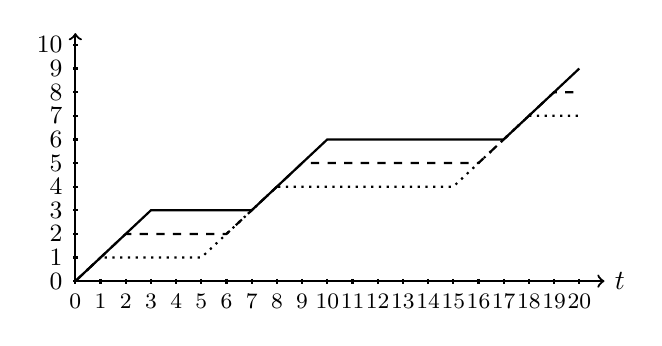
\begin{tikzpicture}[x=\ux,y=\uy, font=\sffamily,thick]  
		\draw[->] (0,0) -- coordinate (xaxis) (21,0) node[anchor=west] {$t$};
		\foreach \x in {0,...,20}{
			\draw[-](\x,0.1) -- (\x,-0.1)
			node[below] {\footnotesize $\x$};
			
		}
		\draw[->] (0,0) node[anchor=east] {}-- coordinate (xaxis) (0,10.5);
		\foreach \y in {0,...,10}{
			\draw[-](0.1, \y) -- (-0.1, \y)
			node[left] {\small $\y$};
			
		}

                \draw[-,thick] (0, 0) -- (3, 3) -- (7, 3) -- (10, 6) -- (17, 6) -- (20, 9);
                \draw[-,dashed] (0 ,0) -- (2,2) -- (6, 2) -- (9, 5) -- (16, 5) -- (19, 8) -- (20, 8);
                \draw[-,dotted] (0, 0) -- (1, 1) -- (5, 1) -- (8, 4) -- (15, 4) -- (18, 7) -- (20, 7);
		\end{tikzpicture}    
  \caption{The workload function $\widehat{W}_j^0(\Delta, c_j^*)$ when $T_j=10$, $C_j=3$, and $D_j=6$. Solid line: $c_j^*$ is $3$, Dashed line: $c_j^*$ is $2$, Dotted line: $c_j^*$ is $1$.}
  \label{fig:example-lemma-workload}
\end{figure}